\documentclass[tikz,border=10pt]{standalone}
\usepackage{tikz}
\usetikzlibrary{shapes,arrows,positioning,calc,patterns,shadows,arrows.meta}

\definecolor{bertblue}{RGB}{66,133,244}
\definecolor{gptgreen}{RGB}{52,168,83}
\definecolor{clsorange}{RGB}{251,188,5}
\definecolor{sepviolet}{RGB}{142,36,245}

\begin{document}
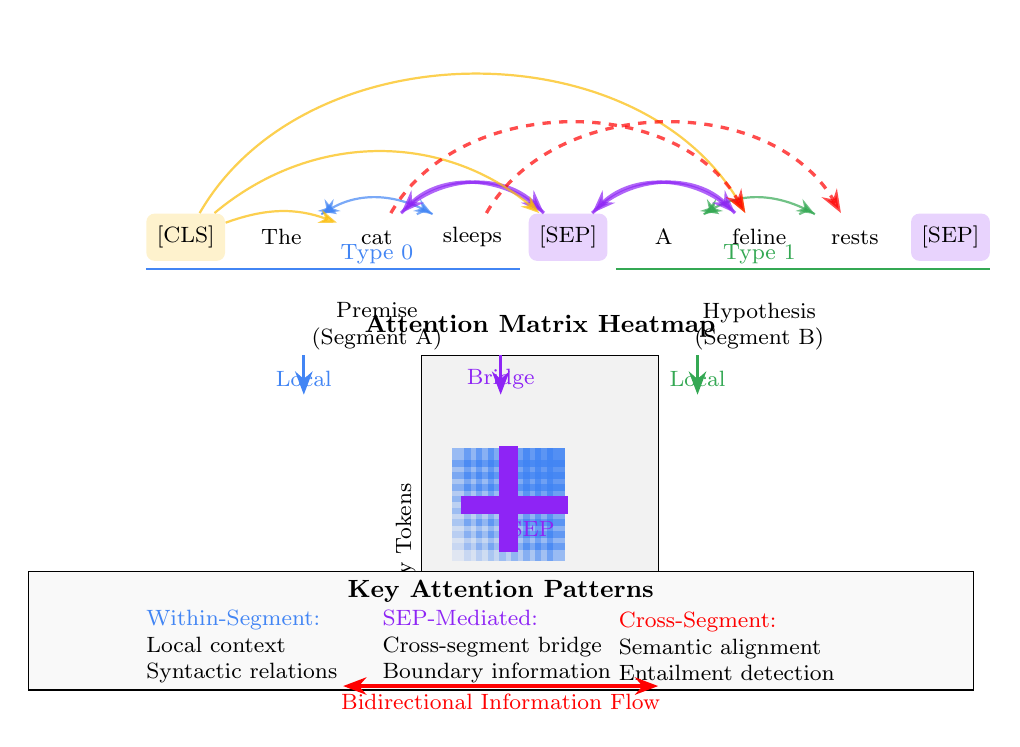
\begin{tikzpicture}[
    token/.style={rectangle, rounded corners=3pt, minimum width=1cm, minimum height=0.6cm, font=\footnotesize},
    attention/.style={-{Stealth}, thick, opacity=0.7},
    label/.style={font=\footnotesize}
]

% === SPACING AND ALIGNMENT DOCUMENTATION ===
% Token row: y=6, spaced 1cm apart horizontally
% Segment labels: y=5.3
% Segment type indicators: y=5.5-5.7
% Attention matrix: centered at (4, 3.5)
% Key patterns table: y=1
% Information flow: y=0.3

% Input sequence for NLI task - using relative positioning
\node[token, fill=clsorange!20] (cls) at (0, 6) {[CLS]};
\node[token, fill=white, right=0.2cm of cls] (t1) {The};
\node[token, fill=white, right=0.2cm of t1] (t2) {cat};
\node[token, fill=white, right=0.2cm of t2] (t3) {sleeps};
\node[token, fill=sepviolet!20, right=0.2cm of t3] (sep1) {[SEP]};
\node[token, fill=white, right=0.2cm of sep1] (t4) {A};
\node[token, fill=white, right=0.2cm of t4] (t5) {feline};
\node[token, fill=white, right=0.2cm of t5] (t6) {rests};
\node[token, fill=sepviolet!20, right=0.2cm of t6] (sep2) {[SEP]};

% Segment labels - positioned relative to tokens
\node[label, align=center, below=0.4cm of t2] {Premise\\(Segment A)};
\node[label, align=center, below=0.4cm of t5] {Hypothesis\\(Segment B)};

% Segment type indicators - properly aligned with segments
\draw[thick, bertblue] ($(cls.south west)+(0,-0.1)$) -- ($(sep1.south west)+(-0.1,-0.1)$);
\draw[thick, gptgreen] ($(sep1.south east)+(0.1,-0.1)$) -- ($(sep2.south east)+(0,-0.1)$);
\node[label, bertblue, above] at ($(t2.south)+(0,-0.15)$) {Type 0};
\node[label, gptgreen, above] at ($(t5.south)+(0,-0.15)$) {Type 1};

% Self-attention within segments
% Premise self-attention
\draw[attention, bertblue, bend left=30] (t1) to (t2);
\draw[attention, bertblue, bend left=30] (t2) to (t3);
\draw[attention, bertblue, bend right=30] (t3) to (t1);

% Hypothesis self-attention  
\draw[attention, gptgreen, bend left=30] (t4) to (t5);
\draw[attention, gptgreen, bend left=30] (t5) to (t6);
\draw[attention, gptgreen, bend right=30] (t6) to (t4);

% Cross-segment attention through SEP
\draw[attention, sepviolet, very thick, bend left=45] (t2) to (sep1);
\draw[attention, sepviolet, very thick, bend left=45] (sep1) to (t5);
\draw[attention, sepviolet, very thick, bend right=45] (t5) to (sep1);
\draw[attention, sepviolet, very thick, bend right=45] (sep1) to (t2);

% CLS attention to both segments
\draw[attention, clsorange, bend left=20] (cls) to (t2);
\draw[attention, clsorange, bend left=40] (cls) to (sep1);
\draw[attention, clsorange, bend left=60] (cls) to (t5);

% Cross-segment semantic connections
\draw[attention, red, dashed, very thick, bend left=60] (t2) to (t5);
\draw[attention, red, dashed, very thick, bend left=60] (t3) to (t6);

% Attention matrix visualization - positioned below tokens
\node[rectangle, draw=black, fill=gray!10, minimum width=3cm, minimum height=3cm] (matrix) at (4.5, 3) {};
\node[font=\small\bfseries, above=0.1cm of matrix.north] {Attention Matrix Heatmap};

% Create grid for attention visualization - smaller and better positioned
\foreach \i in {0,...,8} {
    \foreach \j in {0,...,8} {
        \pgfmathsetmacro{\opacityval}{0.1 + 0.05*(\i+\j)}
        \pgfmathsetmacro{\xpos}{3.5+\i*0.15}
        \pgfmathsetmacro{\ypos}{2+\j*0.15}
        \node[rectangle, fill=bertblue, opacity=\opacityval, minimum size=0.2cm] at (\xpos, \ypos) {};
    }
}

% Highlight SEP attention patterns
\node[rectangle, fill=sepviolet, minimum width=0.2cm, minimum height=1.35cm] at (4.1, 2.675) {};
\node[rectangle, fill=sepviolet, minimum width=1.35cm, minimum height=0.2cm] at (4.175, 2.6) {};

% Labels for attention matrix
\node[label, rotate=90, left=0.2cm of matrix.west] {Query Tokens};
\node[label, below=0.2cm of matrix.south] {Key Tokens};
\node[label, sepviolet] at (4.4, 2.3) {SEP};

% Key observations
\node[rectangle, draw=black, fill=gray!5, minimum width=12cm, minimum height=1.5cm] at (4, 1) {};
\node[font=\small\bfseries] at (4, 1.5) {Key Attention Patterns};

\node[label, align=left, text width=3cm] at (1, 0.8) {\textcolor{bertblue}{Within-Segment:}\\Local context\\Syntactic relations};
\node[label, align=left, text width=3cm] at (4, 0.8) {\textcolor{sepviolet}{SEP-Mediated:}\\Cross-segment bridge\\Boundary information};
\node[label, align=left, text width=3cm] at (7, 0.8) {\textcolor{red}{Cross-Segment:}\\Semantic alignment\\Entailment detection};

% Information flow arrows
\draw[-{Stealth}, very thick, bertblue] (1.5, 4.5) -- (1.5, 4);
\node[label, bertblue] at (1.5, 4.2) {Local};

\draw[-{Stealth}, very thick, sepviolet] (4, 4.5) -- (4, 4);
\node[label, sepviolet] at (4, 4.2) {Bridge};

\draw[-{Stealth}, very thick, gptgreen] (6.5, 4.5) -- (6.5, 4);
\node[label, gptgreen] at (6.5, 4.2) {Local};

% Bidirectional flow indicator
\draw[{Stealth}-{Stealth}, very thick, red] (2, 0.3) -- (6, 0.3);
\node[label, red] at (4, 0.1) {Bidirectional Information Flow};

\end{tikzpicture}
\end{document}